\documentclass[a4paper]{article}
\usepackage{tikz}
\usetikzlibrary{shapes, arrows, positioning}

%% pdflatex network_diagram_sample.tex && rm *.aux *.log

% Définition des styles pour les logos
\tikzset{
    server/.style={rectangle, draw=black, fill=blue!20, text width=5em, text centered, rounded corners, minimum height=2em},
    terminal/.style={rectangle, draw=black, fill=green!20, text width=5em, text centered, rounded corners, minimum height=2em},
    router/.style={diamond, draw=black, fill=red!20, text width=5em, text centered, minimum height=2em},
    firewall/.style={ellipse, draw=black, fill=yellow!20, text width=5em, text centered, minimum height=2em},
    ai/.style={circle, draw=black, fill=purple!20, text width=5em, text centered, minimum height=2em},
    communication/.style={trapezium, draw=black, fill=cyan!20, text width=5em, text centered, minimum height=2em},
    data_center/.style={regular polygon, regular polygon sides=6, draw=black, fill=orange!20, text width=5em, text centered, minimum height=2em},
    iot/.style={rectangle, draw=black, fill=teal!20, text width=5em, text centered, minimum height=2em},
    storage/.style={cylinder, draw=black, fill=brown!20, text width=5em, text centered, shape aspect=0.2, minimum height=2em, shape border rotate=90},
    control/.style={star, draw=black, fill=magenta!20, text width=5em, text centered, minimum height=2em},
    mainframe/.style={rectangle, draw=black, fill=gray!20, text width=5em, text centered, minimum height=4em},
    security/.style={ellipse, draw=black, fill=black!20, text=white, text width=5em, text centered, minimum height=2em},
    virtualization/.style={rectangle, draw=black, fill=lime!20, text width=5em, text centered, minimum height=2em},
    vpn/.style={rectangle, draw=black, fill=pink!20, text width=5em, text centered, minimum height=2em},
    line/.style={draw, -latex'}
}

\begin{document}

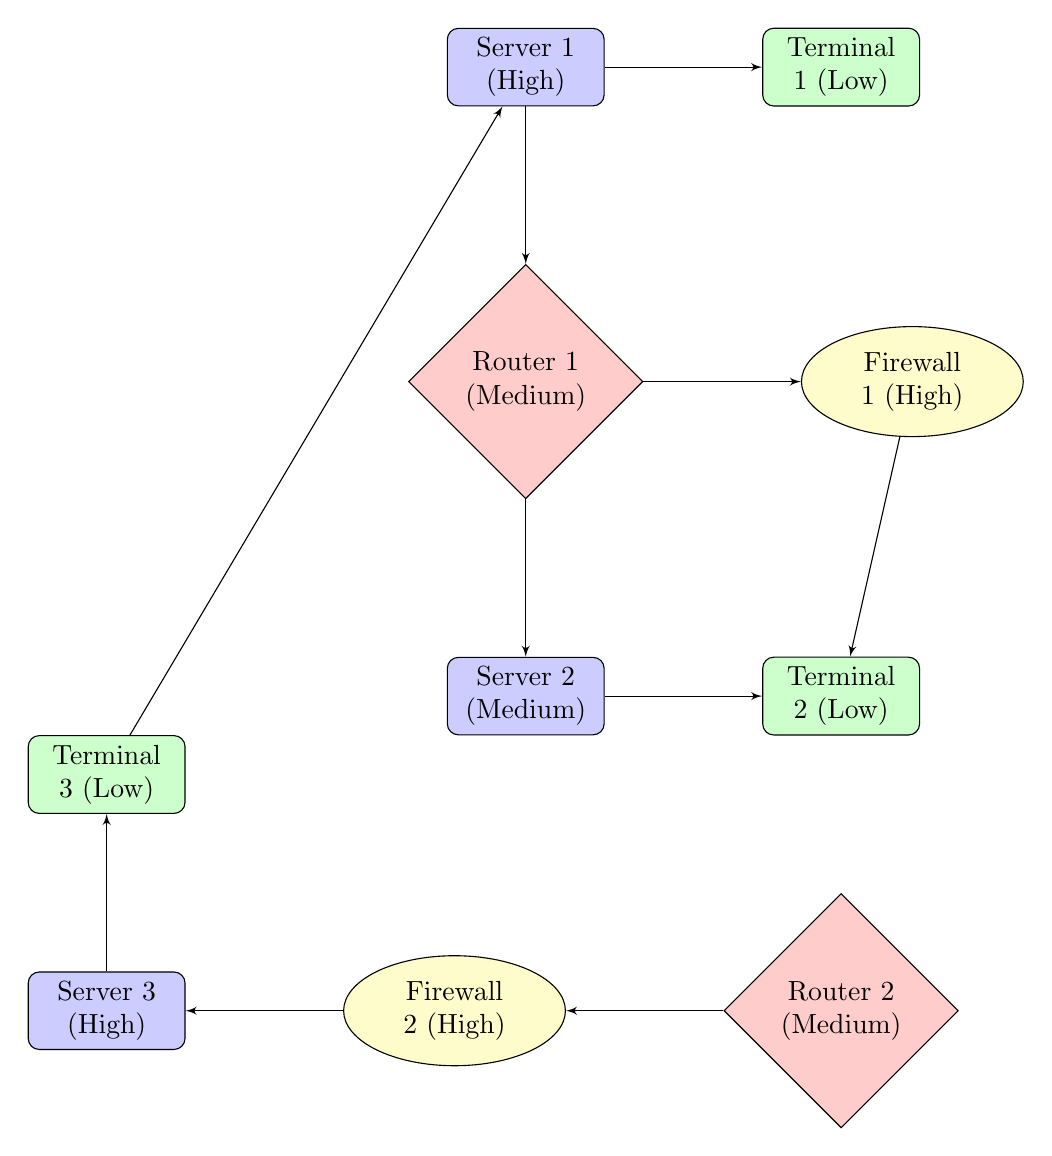
\begin{tikzpicture}[node distance=2cm, auto]

    % Nodes
    \node [server] (Server1) {Server 1 (High)};
    \node [terminal, right=of Server1] (Terminal1) {Terminal 1 (Low)};
    \node [router, below=of Server1] (Router1) {Router 1 (Medium)};
    \node [firewall, right=of Router1] (Firewall1) {Firewall 1 (High)};
    \node [server, below=of Router1] (Server2) {Server 2 (Medium)};
    \node [terminal, right=of Server2] (Terminal2) {Terminal 2 (Low)};
    \node [router, below=of Terminal2] (Router2) {Router 2 (Medium)};
    \node [firewall, left=of Router2] (Firewall2) {Firewall 2 (High)};
    \node [server, left=of Firewall2] (Server3) {Server 3 (High)};
    \node [terminal, above=of Server3] (Terminal3) {Terminal 3 (Low)};

    % Connections
    \path [line] (Server1) -- (Terminal1);
    \path [line] (Server1) -- (Router1);
    \path [line] (Router1) -- (Firewall1);
    \path [line] (Firewall1) -- (Terminal2);
    \path [line] (Router1) -- (Server2);
    \path [line] (Server2) -- (Terminal2);
    \path [line] (Router2) -- (Firewall2);
    \path [line] (Firewall2) -- (Server3);
    \path [line] (Server3) -- (Terminal3);
    \path [line] (Terminal3) -- (Server1);

\end{tikzpicture}

\end{document}
